\documentclass[a4paper, twocolumn, 10pt]{jarticle}
\usepackage[dvipdfmx]{graphicx}
\usepackage[dvipdfmx]{color}
\usepackage{float}
\usepackage{setspace}
\usepackage[top=20mm,bottom=20mm,left=23mm,right=23mm]{geometry}
\usepackage[hang,small,bf]{caption}
\usepackage{bm}

\usepackage{comment}
%\usepackage[subrefformat=parens]{subcaption}
% \usepackage{jumoline}
\usepackage[hyphens]{url}
\usepackage[dvipdfmx, bookmarkstype=toc, colorlinks=false, pdfborder={0 0 0}, bookmarks=true, bookmarksnumbered=true]{hyperref}
\usepackage{pxjahyper}
\usepackage{here}
\usepackage{otf}
\usepackage{amsmath}

\makeatletter

\def\section{%
	\@startsection{section}{1}{\z@}%
	{.1\Cvs \@plus.1\Cdp \@minus.1\Cdp}%
	{.1\Cvs \@plus.1\Cdp}%
	{\normalfont\normalsize\bfseries}%
}

\def\subsection{%
	\@startsection{subsection}{1}{\z@}%
	{.1\Cvs \@plus.1\Cdp \@minus.1\Cdp}%
	{.1\Cvs \@plus.1\Cdp}%
	{\normalfont\normalsize\bfseries}%
}

\def\@maketitle {
	\begin{center}
		\fontsize{14pt}{0pt}\selectfont
		{\bf \@title}
	\end{center}
	\vspace{1pt}
	\begin{flushleft}
		{指導教員 木村 昌臣}\hfill{片岡 凪}
	\end{flushleft}
	\vspace{10pt}
}

\makeatother

\captionsetup{compatibility=false}
\pagestyle{empty}


\begin{document}

\title{主張と根拠のクラスタを用いた多様な主張を提示するニュース推薦手法の提案}

\maketitle

\thispagestyle{empty}

%%%%%%%%%%%%%%%%%%%%%%%%%%%%%%%%%%%%%%%%%%%
%% Section 研究の背景と目的
%%%%%%%%%%%%%%%%%%%%%%%%%%%%%%%%%%%%%%%%%%%
\section{研究の背景と目的}

ニュース記事となる出来事は,記者によって受け取り方や伝え方が異なる.
RSF(Reporters Sans Frontières)は,政治や文化などの要因によって記者の主張が制限されていることを問題視している\cite{2021_world_press_freedom_index}.
近年のWebニュースには世界中の記者たちの様々な主張が散見されるが,言語の違いによる時間的コストなどから,多くの読者はそれらの主張の一部しか把握できない.

Yangらは,ニュース読者が出来事を正確かつ迅速に把握できるように,
階層的クラスタリングを用いて記事に対するツイートの主張をグループ化する手法を提案した\cite{yang_scalable_2021}.
この研究ではCOVID-19の話題に限定した主張の文をグループ化しているが,この手法をWeb上の\textcolor{red}{多く}の話題の記事に適用した場合,\textcolor{red}{多く}の話題の主張のグループが生成されることになる.
% 1度のクラスタリングで
% 無数の主張のグループが生成されることになる.
これでは,COVID-19の
\textcolor{red}{飲み薬やワクチンといった異なる話題から安全性に関する共通した}
% ワクチンに対する主張と脳炎のワクチンに対する
主張が\textcolor{red}{■}
% 近くに
グループ化される\textcolor{red}{ような}事が起き得るため,同じ出来事の異なる主張の収集に時間を要してしまう.
% これにより,ニュース読者の正確かつ迅速な出来事の把握の支援を目指す.
% 異なる話題の似た主張をグループ化するエラーに繋がりやすいと考えられる.

% ワクチン 感染 病床 旅行 政治 制作 感染者数 症状 副反応
% 安全性 危険性 予防 

% 近いグループに正確さ
% カテゴリをCOVID-19に限定させたニュースだけでも
% ノイズとなり得る
% Web上には世界の無数の記事には対応できない
% クラスタ数がいうほど減っていない



% より近い出来事を

そこで本研究では,まず世界の記事を出来事の類似度に基づいてグループ化し,同じグループの記事群から主張の類似度に基づいて再度グループ化することにより,より類似した出来事の異なる主張の文を推薦する手法を提案する.
% これにより,ニュース読者の正確かつ迅速な出来事の把握の支援を目指す.
% ここで,「出来事」は記者の解釈に依存しない事象とし,「主張」は記者が伝えるべきだと判断した出来事の解釈とする.


%%%%%%%%%%%%%%%%%%%%%%%%%%%%%%%%%%%%%%%%%%%
%% Section 関連研究
%%%%%%%%%%%%%%%%%%%%%%%%%%%%%%%%%%%%%%%%%%%
% \section{関連研究}
% 意味や話題が類似する文章の推薦手法として,LDA(Latent Dirichlet Allocation)~\cite{tian_labeled_2018}やSentence-BERT~\cite{reimers_sentence-bert_2019}が提案されている.
% LDAは記事に関連の深い単語群とそれぞれの単語の関連度を出力するが,単語群同士の関係性が得られないという点で,出来事の類似度が高い記事は得にくいと考えられる.
% 一方,Sentence-BERTは単語同士の関係性を加味した文意の数値ベクトルを出力するため,より高い出来事の類似度が得られると考えられる.
% しかし,記事の全文をSentence-BERTに入力した場合,出来事の類似度の算出に主張を述べる文も考慮することになり,より近い出来事に関する主張の違いを推薦できない.

% \begin{comment}
% SCDV, オントロジー, Transformer
% 潜在的意味,同義語
% トピック同士の関係が考慮されない
% 多言語に対応していない
% 主張に着目した研究は少ない
% 事象と主張が混在
% \end{comment}

% \begin{table}[h]
%   \caption{キャプション}
%   \label{table_a}
%   \centering
%   \begin{tabular}{lcr}
%     \hline
%     手法   & 正解率[\%]  &  計算時間[ms]  \\
%     \hline \hline
%     手法A  & 92.3  & 512 \\
%     手法B  & 87.4  & 32  \\
%     \hline
%   \end{tabular}
% \end{table}

%%%%%%%%%%%%%%%%%%%%%%%%%%%%%%%%%%%%%%%%%%%
%% Section 提案手法
%%%%%%%%%%%%%%%%%%%%%%%%%%%%%%%%%%%%%%%%%%%

\section{提案手法}
図\ref{system_abstract}に提案手法の概要を示す.
まず
\textcolor{red}{(\ajroman{1})}
記事の文章を出来事の文と主張の文に分類し,
次に
\textcolor{red}{(\ajroman{2})}
出来事の文章の類似度で記事をクラスタリングし,
その後
\textcolor{red}{(\ajroman{3})}
主張の文の類似度で主張の文をクラスタリングする.

\begin{figure}[H]
	\centering
	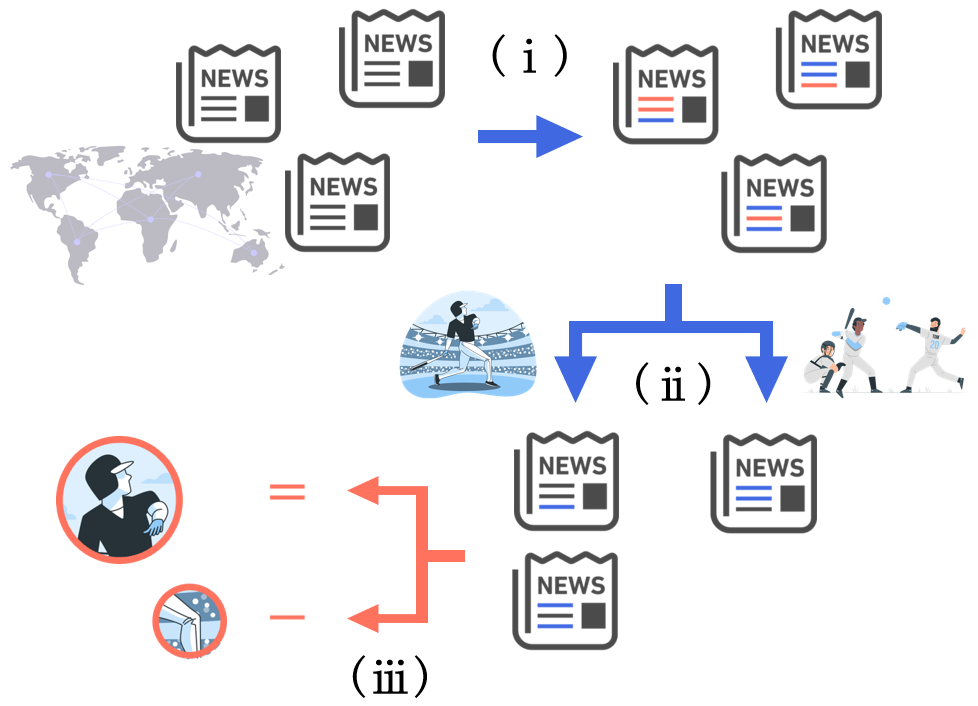
\includegraphics[keepaspectratio, width=60mm]{img/system_abstract.png}
	\caption{
    提案手法の概要
  }
	\label{system_abstract}
\end{figure}

% \subsection{データセットの選定と前処理}
\subsection{RoBERTaによる出来事の文と主張の文の分類}
入力する記事には,Piyushらが収集したCOVID-19 News Articlesを選定した\cite{ghasiya_investigating_2021}.
COVID-19はフェイクニュースが多い話題であり,またインド,日本,韓国の
約8万件
% 47342+21039+10076=78457
の英記事が含まれるため,政治や文化の違いに由来する多くの異なる主張が分析できると考えた.
また,11カ月間という短い期間で収集されているため,より類似した出来事に関する記事が得られると
\textcolor{red}{期待できる.}
% 考えた.
% 省略可能?
Yangらの研究と同様に話題がCOVID-19に限定されてしまっているが,限定された話題でも同じ出来事の異なる主張がグループ化される様子は観測できると考えた.
% @see weekly-report_20210930.md

% このとき
% また,記事の出来事をより類似させるため,同じ出稿日の記事を扱う.
% の各文章が,出来事と主張のどちらを述べているかを分類する.
本研究では,記事の文章が出来事を述べる文と主張を述べる文に二分できると仮定する.
% そして,出来事の文のみ,主張の文のみで2回に分けてクラスタリングすることで,より近い出来事に関する異なる主張の文の推薦を目指す.
出来事と主張の文の分類には,RoBERTaを転移学習した分類器を用いる.
RoBERTaは文意や文脈を加味した自然言語処理が可能な機械学習モデルで\textcolor{red}{ある}
% ,GLUE,SQuAD,RACEといったベンチマークで2019年の最先端のスコアを有している
\cite{liu_roberta_2019}.
\textcolor{red}{事前学習モデルには,}ニュース記事を含む約160GBの文章データ
% で事前に学習された
\textcolor{red}{を学習した}
RoBERTa BASEモデルを利用し\textcolor{red}{た.}
% ,これが出来事と主張の分類に適用できるよう,出来事か主張かでラベル付けした文で追加の学習を行った.
% 学習の活性化関数には???を,損失関数には交差エントロピーを用いた.
% で,Dense層を加えたモデルのエンコード部分を用いることで分類タスクに応用できる.
% 入力部分にDense層を付加

追加学習には,Wikipediaの英文をClaimを述べるかEvidenceを述べるかでラベル付けしたRutyらのIBM Debater$^{\textregistered}$ - Claims and Evidenceを利用した\cite{rinott_show_2015}.
2294個のClaimは「トピックを直接サポートする一般的で簡潔な文」,
4692組のEvidenceは「トピックの文脈の中でClaimを直接サポートする文章」
と定義されており,本研究では主張とClaim,出来事とEvidenceを同じ定義で扱う.
\textcolor{red}{■■}

% 表\ref{claim_evidence_example}にClaimとEvidenceの例を示す.

% データの数が不均衡であるため,Evidenceの学習の重みに$\frac{2294}{4692}$を乗算し,Evidenceを学習しにくくした.
% 学習の損失関数には交差エントロピーを使用した.

% \begin{table}[H]
%   \caption{IBM Debater$^{\textregistered}$ - Claims and Evidencでラベル付けされたClaimの文(C)とEvidenceの文(E)の例}
%   \centering
%   \begin{tabular}{llp{6cm}}
%     \hline
%     C & global carbon emissions are caused by de-
%     \\
%     & forestation
%     % コンマがないのはデフォルト
%     \\
%     E & From 1990 to 2010 Nigeria nearly halved
%     \\
%     & their amount of Forest Cover, moving from
%     \\
%     & 17,234 to 9041 hectares.
%     \\
%     \hline
%   \end{tabular}
%   \label{claim_evidence_example}
% \end{table}

% システム全体の精度向上のため,2つのデータセットの前処理として
% % 正規表現を用いた
% 小文字化やURLの除去などを行った.
% また,文章中の文の区切り位置を同定するため,機械学習ライブラリStanzaによるテキスト解析を行った\cite{qi_stanza_2020}.
% 本システムにおいてStanzaはルールベースのspaCyよりも高速で,句点と句点以外のピリオドを精度良く区別できることを確認した.
% % 省略可能
% % StanzaはルールベースのspaCyに比べ,コンマに強い


%%%%%%%%%%%%%%%%%%%%%%%%%%%%%%%%%%%%%%%%%%%

\subsection{
Sentence-BERT,コサイン\textcolor{red}{値},Ward法を用いた
出来事と主張の
階層的クラスタリング
% による出来事の文章と主張の文のグループ化
}

「出来事と分類した文を記事ごとに結合した文章」と「主張と分類した文」のそれぞれを,Sentence-BERTを用いて\textcolor{red}{■}
% 機械が解釈しやすい数
ベクトルに変換した.
Sentence-BERTは文章を文意を加味した\textcolor{red}{■}
% 数
ベクトルに変換できる機械学習モデルで\textcolor{red}{ある.}
% ,RoBERTaで65時間かかっていた文の類似度算出を約5秒に短縮し,STSタスク(Semantic Textual Similarity tasks)で2019年の最先端のスコアを有している\cite{reimers_sentence-bert_2019}.
事前に学習されたSentence-BERTのモデルには
% ,ライブラリにデフォルトで提供されている
Nils\textcolor{red}{ら}が公開しているparaphrase-MiniLM-L6-v2を使用した.
% 省略可能

文章間の
% 非類似度
\textcolor{red}{距離}の算出には
% Sentence-BERTの論文で用いられていた
\textcolor{red}{ベクトル間の}コサイン\textcolor{red}{値}
% 距離
を使用し,
% (Ward法について調べたこと,Ward法以外を試せたらそれについて書く)
クラスタ間の
% 非類似度
\textcolor{red}{距離}の算出にはWard法を用いた.
本研究ではより類似した出来事で異なる主張\textcolor{red}{を}得るために,
具体的で有限個存在する出来事の文章\textcolor{red}{に基づいて記事}を先にクラスタリングし,
\textcolor{red}{得られた各クラスタについて}一般的で
% 無数
\textcolor{red}{複数}の出来事と対応する主張の文を\textcolor{red}{抽出して}クラスタリングした.


%%%%%%%%%%%%%%%%%%%%%%%%%%%%%%%%%%%%%%%%%%%
%% Section 実験
%%%%%%%%%%%%%%%%%%%%%%%%%%%%%%%%%%%%%%%%%%%
\section{実験}

\subsection{出来事の文と主張の文の分類器の調整と評価}

% 分類器の学習では,IBM Debater$^{\textregistered}$ - Claims and Evidenceの8割を訓練用,2割をテスト用に分割して評価を行った.
% 学習は全データを40文ごと\textcolor{red}{のバッチ}
% GPUが許す限り大きくした
% RoBERTaの論文にバッチサイズは大きいほど良いとの記載
% 一般の学習ではバッチサイズが大きすぎると収束しにくい
% イテレーション数 128回
% バッチサイズはそれぞれ40文, 10文
% に分割して行い,評価は全データの学習回数(エポック数)ごとに行った.
% また,
\textcolor{red}{■分類器の}
COVID-19 News Articlesでの分類精度を確認するため,
% IBM Debater$^{\textregistered}$ - Claims and Evidenceのラベル付けの傾向を
COVID-19 News Articlesの\textcolor{red}{各}国から3\textcolor{red}{件}の記事\textcolor{red}{■}を抽出し,\textcolor{red}{計163個の文を出来事か主張かで手動で}ラベル付けし,分類器で付与したラベルとの比較評価を行った.
評価指標には,
\textcolor{red}{分類数が少なかった主張の文に着目して■}
% 正しく主張の文と判断した数(TP),
% 正しく出来事の文と判断した数(TN),
% 誤って主張の文と判断した数(FP),
% 誤って出来事の文と判断した数(FN)
% を基に計算した
適合率\textcolor{red}{と}再現率\textcolor{red}{■}
% ,マシューズ相関係数(MCC)
を用いた.
適合率は主張だと判断した文のうち正しく判断できた文の割合,
再現率は主張の文のうち正しく判断できた主張の文の割合を示す.
% MCCは分類器の精度を総合的に評価する指標で,TP,TN,FP,FNが不均衡なときにも頑健に評価できる\cite{chicco_advantages_2020}.
\textcolor{red}{■}
ど\textcolor{red}{ちら}の指標も1に近いことが望ましい.

\textcolor{red}{
  文のラベル付けと分類結果との比較は表\ref{classification_example}のように行った.
  3つ目の文は,一般の大衆にいえる筆者の主張が述べられているが,出来事に誤分類されている.
}
表\ref{classification_evaluation}に評価結果を示す.
\textcolor{red}{
適合率と再現率が共に最大となる3エポック時の分類器が最適であるといえる.
% また,適合率が1であり,主張の文だと判断したときは全て正しく判断できていることがわかる.
■
}
% \textcolor{red}{学習ごとに}損失関数の出力が単調増加していたため,エポック数が大きいと訓練データ以外のデータ
% COVID-19 News Articlesを始めとした一般的なデータ
% で分類精度が悪くなると判断し,少ないエポック数で評価を比較した.
% 省略可能

\begin{table}[H]
  \caption{\textcolor{red}{分類器の主張の文 ($C$)と出来事の文($E$)の分類例}}
  \centering
  {\tabcolsep=0.1cm
  \begin{tabular}{cp{6.5cm}}
      \hline
      分類 & \multicolumn{1}{c}{入力文}
      \\
      \hline
      $C$(正) & the goal was to bolster international competitiveness.
      % 
      % JP69
      % $C$(正) & proponents see the pandemic as a chance to break with the modern calendar.
      % パンデミックは現代のカレンダーと決別するチャンスだと考えています
      % JP42
      \\
      $E$(正) & the government is reportedly aiming to announce guidance early next month.
      % JP81
      % 政府は来月初めにガイダンスを発表することを目指していると言われています
      % $E$(正) & over 20000 people have signed an online petition calling for a shift to september school starts.
      % 9月入学への移行を求めるオンライン署名に2000人以上が参加しました.
      % JP54
      \\
      $E$(誤) & for now there is little that families and educators can do but wait to see what the abe administration has in mind.
      % 今のところ,家族や教育者ができることは,ABE政権が何を考えているかを待つことだけです
      % JP80
      % $E$(誤) & i dont think online classes can completely replace them
      % オンライン授業が完全に代替できるとは思えません.
      % JP60
      \\
      \hline
    \end{tabular}
    \label{classification_example}
    }
\end{table}

\begin{table}[H]
  \caption{
    \textcolor{red}{COVID-19 News Articlesの163文の分類の評価}
    % 使用データとエポック数ごとの
    % 分類器の評価
    % (IBM:IBM Debater$^{\textregistered}$ - Claims and Evidence,News:COVID-19 News Articles)
    }
  \centering
  {\tabcolsep=0.15cm
    \begin{tabular}{ccccp{6cm}}
    \hline
    % データ & 評価指標 & $2$ epochs & $\mathbf{3}$ \textbf{epochs} & $4$ epochs
    \textcolor{red}{■~~}評価指標 & $2$ epochs & $\mathbf{3}$ \textbf{epochs} & $4$ epochs
    \\
    \hline
    % IBM & Loss & $\mathbf{0.21}$ & $0.24$ & $0.30$
    % \\
    % IBM & MCC & $0.82$ & $\mathbf{0.83}$ & $0.82$
    % \\
    % News & TP & $4$ & $\mathbf{6}$ & $5$
    % \\
    % News & TN & $\mathbf{148}$ & $\mathbf{148}$ & $147$
    % \\
    % News & FP & $\mathbf{0}$ & $\mathbf{0}$ & $1$
    % \\
    % News & FN & $11$ & $\mathbf{9}$ & $10$
    % \\
    % News & 適合率 & $\mathbf{1.00}$ & $\mathbf{1.00}$ & $0.83$
    \textcolor{red}{■~~}適合率 & $\mathbf{1.00}$ & $\mathbf{1.00}$ & $0.83$
    \\
    % News & 再現率 & $0.27$ & $\mathbf{0.40}$ & $0.33$
    \textcolor{red}{■~~}再現率 & $0.27$ & $\mathbf{0.40}$ & $0.33$
    \\
    % News & MCC & $0.50$ & $\mathbf{0.61}$ & $0.50$
    % \\
    \hline
    \end{tabular}
  }
  \label{classification_evaluation}
\end{table}


\textcolor{red}{\subsection{2回の階層的クラスタリングの調整と評価}}
クラスタリングの実行時にメモリが不足したため,入力記事は959件に減らした.
図\ref{claim_sentences_dendrogram}に主張の階層的クラスタリングの結果を示す.
クラスタを結合するそれぞれのクラスタ間の距離が一様に分布しており,主張の文意が階層構造を持つことがわかる.
主張の文の推薦に用いる階層のレベルには
% 式(\ref{silhouette_coefficient})に示す
シルエット係数が大きいものを選択した.
この係数が大きいほど同一クラスタ内の文が類似し,異なるクラスタ間の文が類似しないといえる.
% $a(i)$は文$s(i)$と文$s(i)$が属するクラスタの他の文との平均の非類似度であり,$a(i)$が0に近いとクラスタ内の文章がよく凝集しているといえる.
% $b(i)$は文$s(i)$と文$s(i)$の最近傍のクラスタの他の文との平均の非類似度であり,$a(i)$が1に近いと異なるクラスタの文章がよく乖離しているといえる.
% $a(i)$,$b(i)$から得た$Sil(i)$は,1に近いほどよく凝縮と乖離をしているといえる.
% 実験では,分割するクラスタ数ごとに全ての文$s(i)$の$Sil(i)$を計算し,$Sil(i)$の平均$\overline{Sil(i)}$の推移を観察した.
% 必要なメモリ容量が32GBを超えた
% \begin{align}
%   Sil(i) &= \frac{b(i) - a(i)}{\max ( b(i) , a(i))}
%   \label{silhouette_coefficient}
% \end{align}
シルエット係数に基づき,記事を910個のクラスタに分割し,そのうち主張の文を11個持つクラスタの主張の文を9個のクラスタに分割した.
% 図\ref{num_article_clusters_and_silhouette},\ref{num_sentence_clusters_and_silhouette}に示すようにクラスタ数が入力文の数に近いときに$\overline{Sil(i)}$が最大値を取る.


% しかし,読者の迅速な出来事の把握のためには似た文はグループ化したいため,最適なクラスタ数として最大のクラスタ数の95\%以下の領域で$\overline{Sil(i)}$が最大値を取るようなクラスタ数を選択した.
% 図\ref{num_sentence_clusters_and_silhouette}は,この選択に基づいて図\ref{num_article_clusters_and_silhouette}でクラスタ数910,$\overline{Sil(i)} \sim 0.38$となるように出来事の文章のクラスタリングを行った後,主張の文の数が多い1つのクラスタについて主張の文のクラスタリングを行った結果である.

\begin{figure}[H]
	\centering
	% 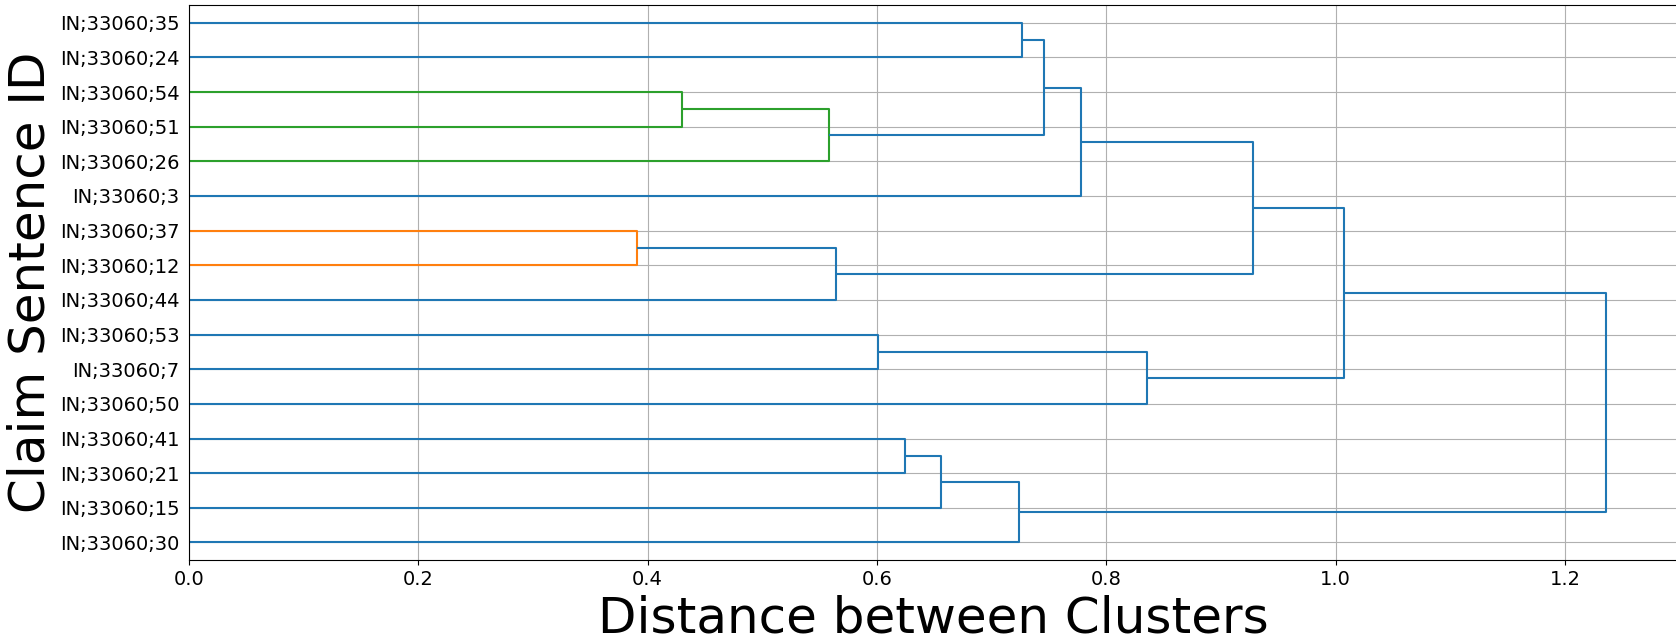
\includegraphics[keepaspectratio, width=60mm]{img/process-07_sentences-cluster_color_dendrogram_reduced-data-to-959_Trim.png}
	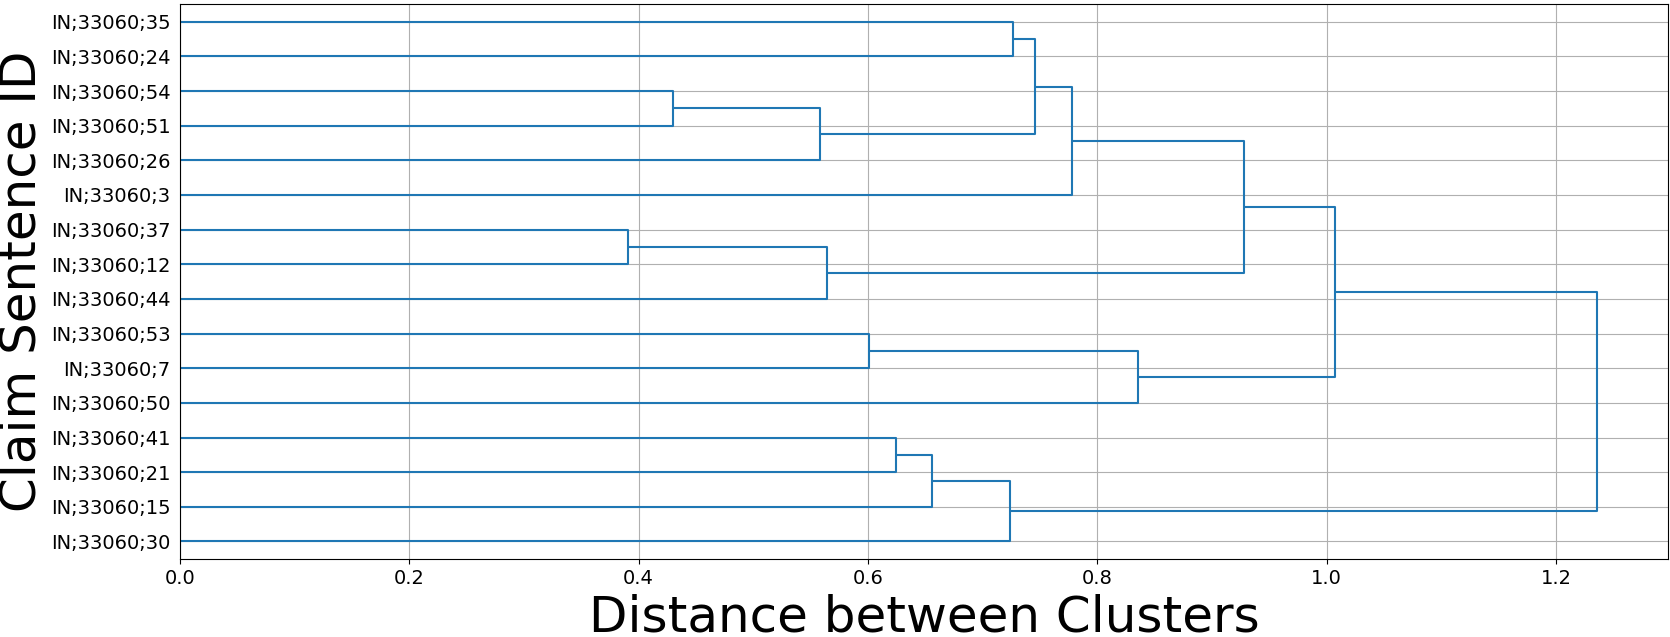
\includegraphics[keepaspectratio, width=60mm]{img/process-07_sentences-cluster_dendrogram_reduced-data-to-959_Trim.png}
	\caption{
    \textcolor{red}{主張の文のクラスタリング結果の可視化}
  }
	\label{claim_sentences_dendrogram}
\end{figure}

% \begin{figure}[H]
% 	\centering
% 	% \includegraphics[keepaspectratio, width=60mm]{img/process-06_articles-cluster_num-of-clusters-dependency-on-silhouette-coefficient_reduced-data-to-5000_Trim.png}
% 	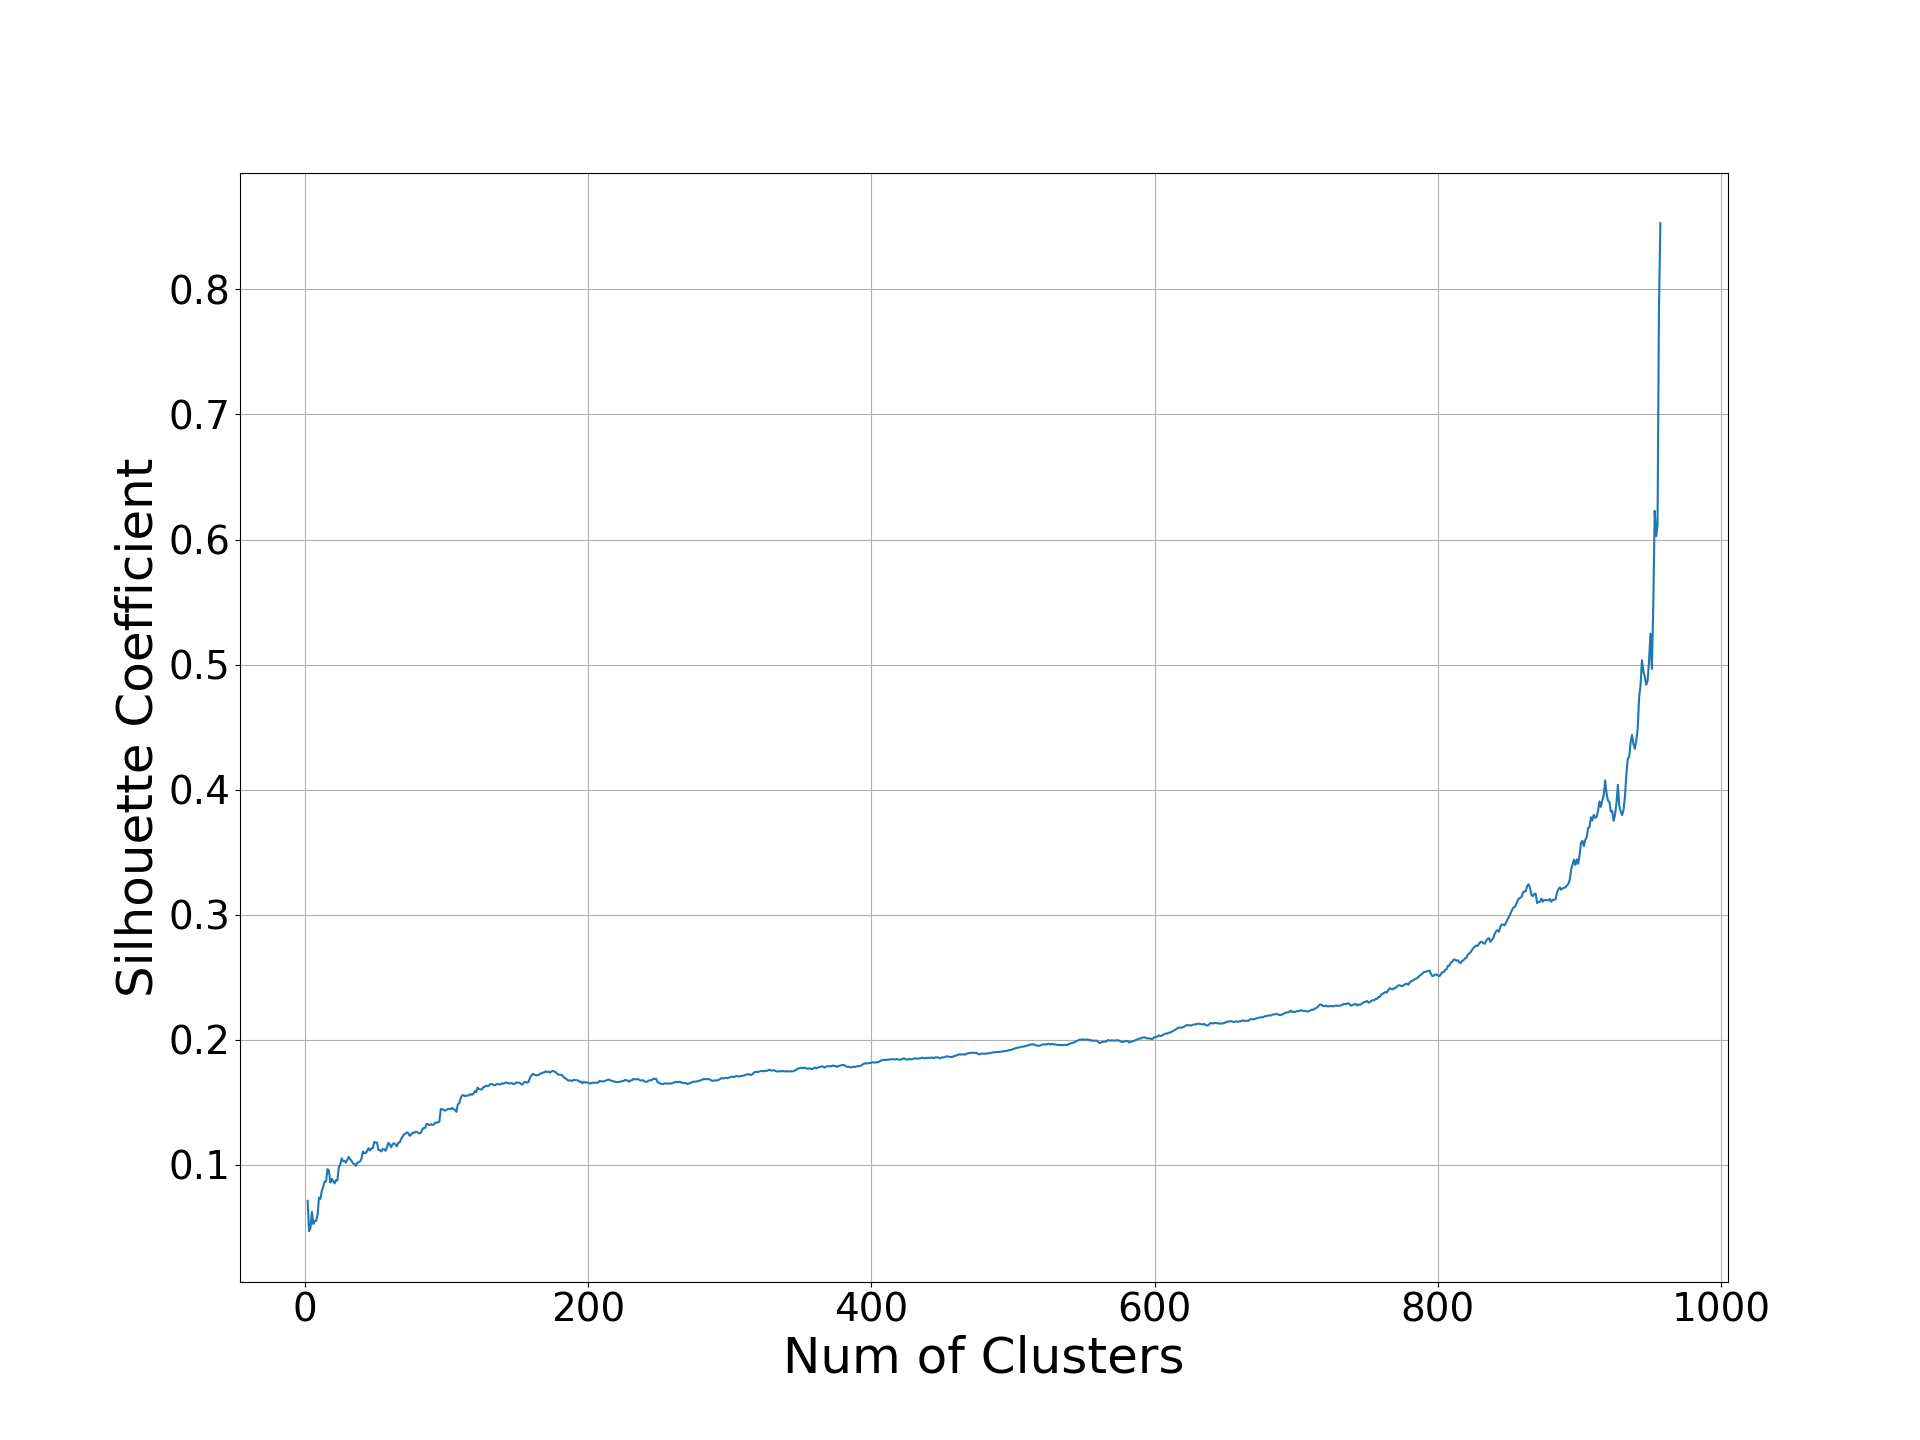
\includegraphics[keepaspectratio, width=60mm]{img/process-06_articles-cluster_num-of-clusters-dependency-on-silhouette-coefficient_with-maximal-silhoette_reduced-data-to-959.png}
% 	\caption{
%     出来事の文章のクラスタ数と$\overline{Sil(i)}$との関係
%   }
% 	\label{num_article_clusters_and_silhouette}
% \end{figure}

% \begin{figure}[H]
% 	\centering
% 	% \includegraphics[keepaspectratio, width=60mm]{img/process-07_sentences-cluster_num-of-clusters-dependency-on-silhouette-coefficient_reduced-data-to-5000_Trim.png}
% 	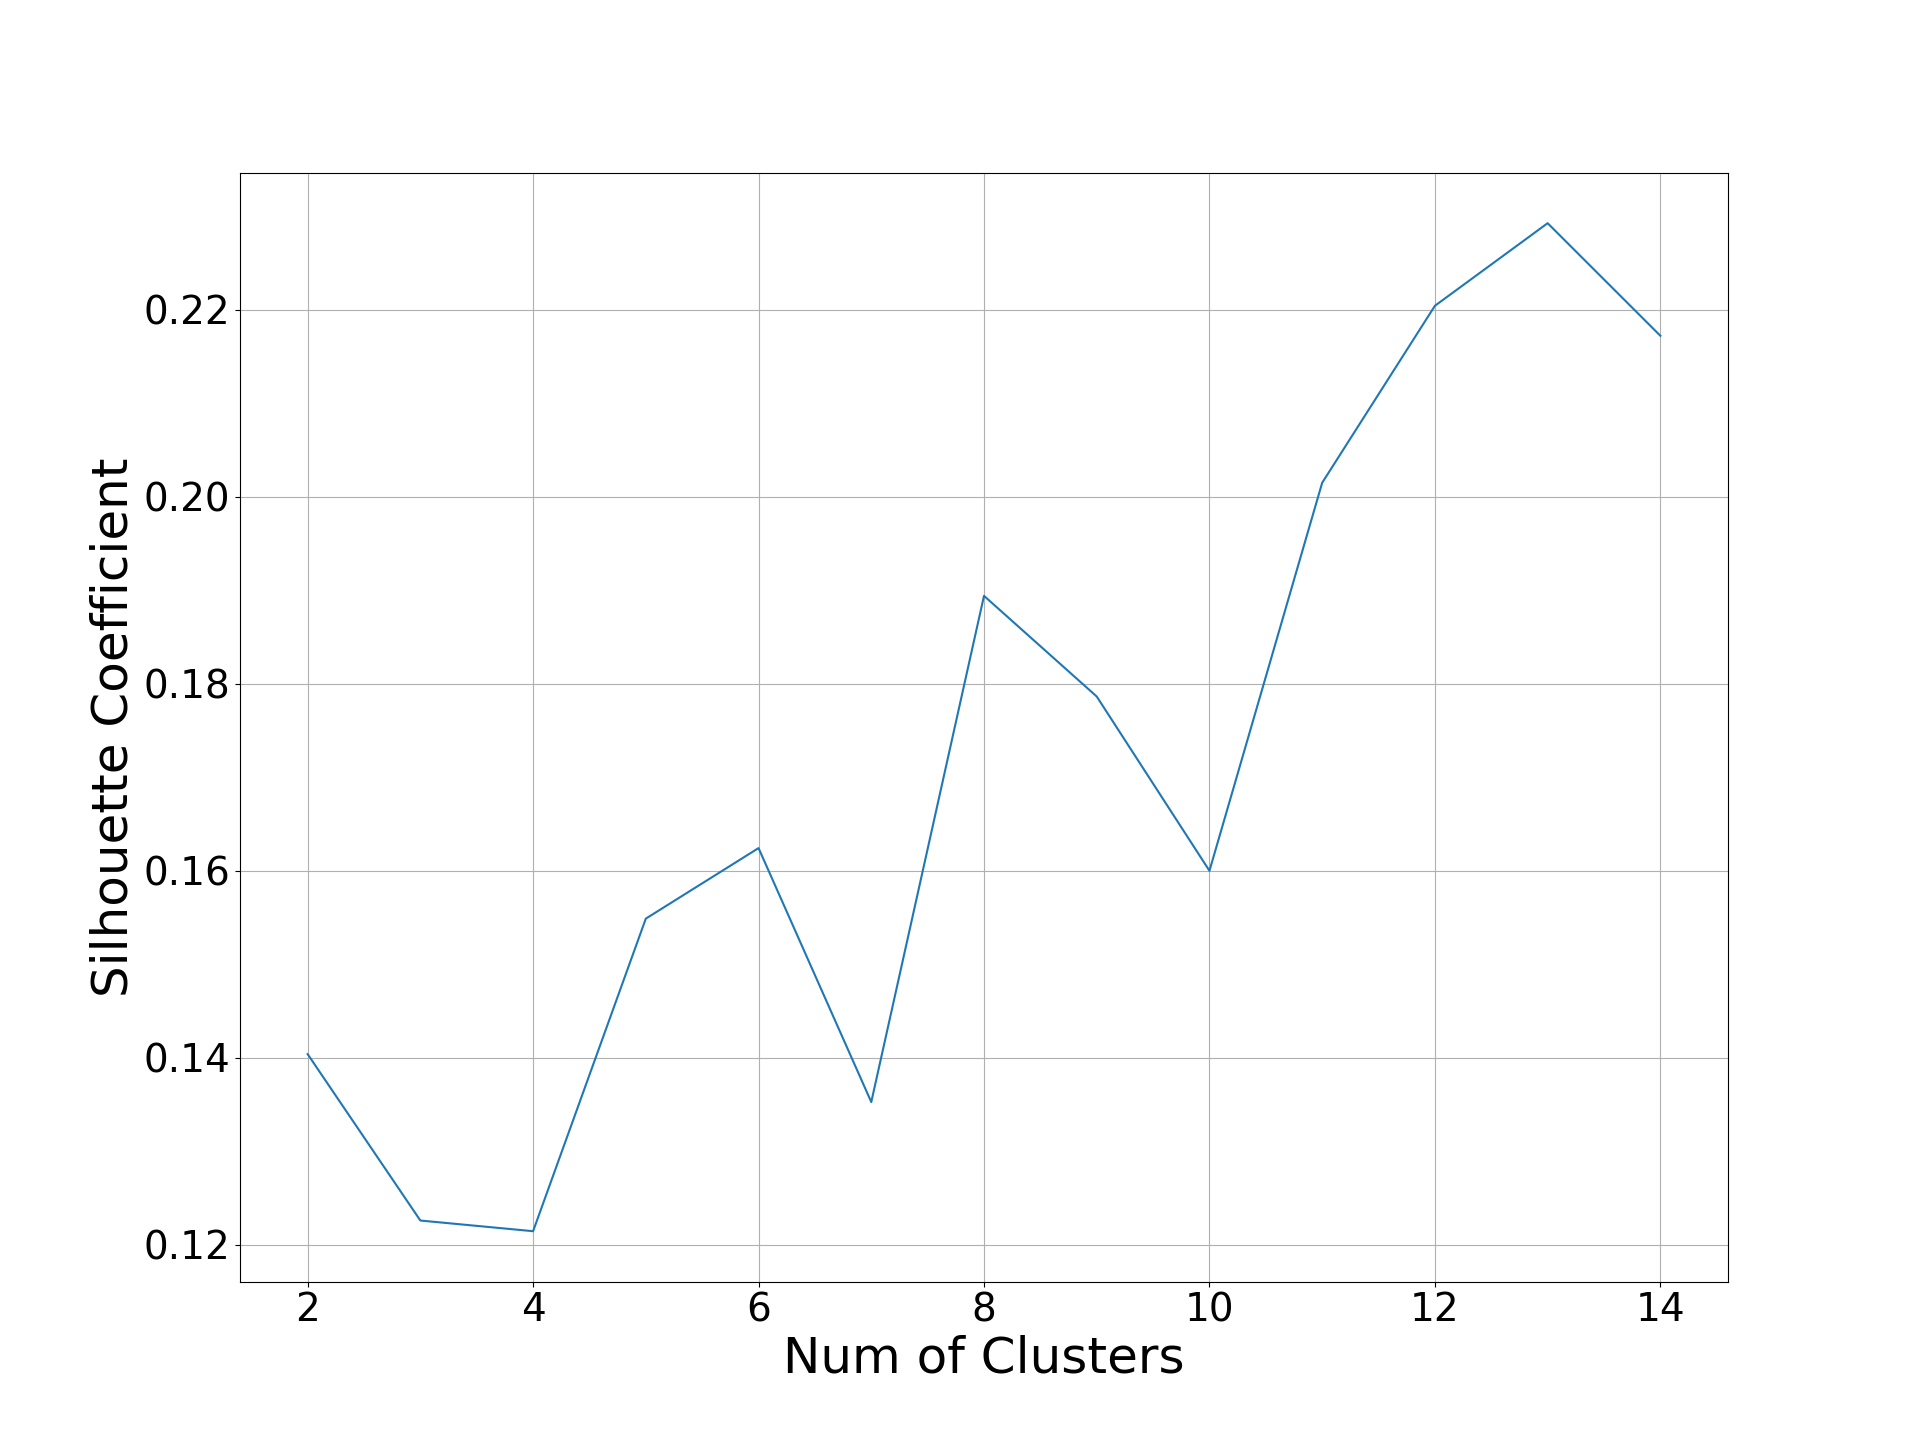
\includegraphics[keepaspectratio, width=60mm]{img/process-07_sentences-cluster_num-of-clusters-dependency-on-silhouette-coefficient_reduced-data-to-959.png}
% 	\caption{
%     主張の文のクラスタ数と$\overline{Sil(i)}$との関係
%   }
% 	\label{num_sentence_clusters_and_silhouette}
% \end{figure}

選択した記事のクラスタには2つの記事が含まれており,どちらもCOVID-19の感染力を話題としていた.
表\ref{clustering_result_samples}に
% 図\ref{num_sentence_clusters_and_silhouette}でクラスタ数13,$\overline{Sil(i)} \sim 0.23$となるように主張の文のクラスタリングを行った結果の一部を示す.
クラスタ内外の主張の文の例を示す.
同じクラスタ$c_1$内には感染力に関する簡潔な主張の文が集まり,それとは別のクラスタ$c_2$には感染力から派生した他の主張の文が配置されていることがわかる.$c_1, c_2$以外のクラスタの8個の文のうち,$c_1$の文と類似してしまった文は2個,$c_1$の文から派生した異なる主張の文は3個,$c_1$の文と関連しない文は3個存在した.$c_1$の文と関連しない文は全て,$c_1$とのクラスタ間距離が大きいクラスタに属していた.
% /** 定量化した主観評価を追加する? **/

\begin{table}[H]
  \caption{
      同じクラスタIDと異なるクラスタIDでの文の比較
    }
  \centering
  {\tabcolsep=0.05cm
    \begin{tabular}{cp{7.5cm}}
    \hline
    ID & \multicolumn{1}{c}{主張の文}
    \\
    \hline
    $c_1$ & it spreads rapidly all over the world and overtakes the people attacking their immune system.
    \\
    $c_1$ & the patient then spreads the disease to others clandestinely.
    \\
    $c_2$ & the chances of similar outbreaks are lower if the virus infects humans and then evolve its highly pathogenic properties.
    \\
    \hline
    \end{tabular}
  }
  \label{clustering_result_samples}
\end{table}

% /**

% (バッチサイズ,エポック数,不均衡データ用のウェイト)

% (IBMからcovidへの適用,IBMのラベルの傾向分析,独自の手付けラベル,不均衡データ用の正例の設定とMCC)


% (クラスタリング結果の文の組の表)

% (hとc?関連研究の相関分析?カイ二乗分布?)


% 分類精度

% 計算時間

% 良く見える結果

% 気になるエラー例

% タイトル回収?

% **/

%%%%%%%%%%%%%%%%%%%%%%%%%%%%%%%%%%%%%%%%%%%
%% Section 考察
%%%%%%%%%%%%%%%%%%%%%%%%%%%%%%%%%%%%%%%%%%%
\section{考察}
表\ref{classification_evaluation}に示すように適合率が極めて大きいため,殆ど正しい主張のみでクラスタリングと推薦を行うことができる.
一方で再現率は低く,本来主張である文をクラスタリングに組み込めない可能性が高い.
しかし,入力記事を増やすことで多くの主張の文を組み込むことができるため,再現率の低さは大きな問題ではない.
入力記事は分散処理によって増やすことが可能である.
なお,主張の文は163文のうち6文しかなかったため,より信頼できる適合率と再現率の算出のためにより多くの文での評価が必要である.

2回のクラスタリングで得られた$c_1$と$c_2$内の記事は互いに異なる記事から構成されており,別の記事から類似した出来事の異なる主張を得ることができたといえる.
その精度は$\frac{4}{9}\sim0.44$であり,クラスタ間距離から絞り込むことで更なる精度の向上が期待できる.
% /**

% 主観評価を被験者を増やして行う

% バッチサイズの改善

% T5の利用の検討

% 良く見える結果->妥当性

% エラーの原因と対策

% タイトル回収?

% 手付けラベルをバイアスのない複数人の被験者で試す

% **/


%%%%%%%%%%%%%%%%%%%%%%%%%%%%%%%%%%%%%%%%%%%
%% Section まとめ
%%%%%%%%%%%%%%%%%%%%%%%%%%%%%%%%%%%%%%%%%%%
\section{まとめ}
本研究では出来事の文と主張の文のクラスタを用いた多様な主張を提示するニュース推薦手法の提案を行った.
提案手法ではより類似した出来事の異なる主張を推薦するため,記事の文を出来事の文か主張の文かで分類し,それぞれの文に基づいて2回の階層的クラスタリングを行った.
その結果,高い適合率で分類を行い,44\%の精度で類似した出来事の異なる主張を推薦できた.
今後の課題として,クラスタ間距離から推薦の精度を向上する必要がある.
% /**

% 手法の目的を1文で説明

% 主にタイトル

% 何をしたか

% 結果何ができたか

% 課題

% **/

% /**

% 参考文献は半分以下に減らす予定

% **/

%%%%%%%%%%%%%%%%%%%%%%%%%%%%%%%%%%%%%%%%%%%
%% Section 研究状況
%%%%%%%%%%%%%%%%%%%%%%%%%%%%%%%%%%%%%%%%%%%
% \section{研究状況}

% 分類精度の確認のため,前述の操作で出来事の文と主張の文の分類を行った.
% ただし,分類する日本の記事にはJapanese FakeNews Dataset中の偽物でないWikinewsを利用した~\cite{japanese_fakenews_dataset}.
% 学習で正解率が約0.993となったモデルで分類を行ったところ,表\ref{classify_result}の結果が得られた.


% \begin{table}[h]
%   \caption{Evidenceの文 ($E$) とClaimの文 ($C$) の分類結果}
%   \label{classify_result}
%   \centering
%   \begin{tabular}{cp{6cm}}
%     \hline
%     分類 & \multicolumn{1}{c}{翻訳前の入力文(一部抜粋)}  \\
%     \hline \hline
%     $E$  & 決勝のヒットを打った23日の試合も1球だけで終わった \\
%     $C$  & 日本シリーズ進出を決めてうれしい \\
%     \hline
%   \end{tabular}
% \end{table}

% 文$E$は,記者の解釈に依存しない,誰が観測しても不変な出来事を表している.
% また,文$C
% % , C_3, C_5
% $は,出来事に対する主張を表している.
% 一方で
% 文中に出来事を表す「敗れた」や「風が吹く」という言葉が含まれることより,出来事を誤分類したケースも見られた.

%%%%%%%%%%%%%%%%%%%%%%%%%%%%%%%%%%%%%%%%%%%
%% Section 今後の予定
%%%%%%%%%%%%%%%%%%%%%%%%%%%%%%%%%%%%%%%%%%%
% \section{今後の予定}

% 今後は,1文中の出来事と主張の要素を比率で考えるなどして,推薦精度を高めるように研究を進める予定である.

% 現在,主張を述べる文章を二重引用符を含む文章と仮定しているが,指示語や否定語の係り受けや引用符内の単語数によってはこの仮定は不適切である可能性がある.
% また,引用符の外の文章も主張を述べる文章である可能性があり,推薦の精度のために精査が必要である.
% 加えて,Transformerに代わるクラスタリング手法として,文意をベクトルで表現するLCDA(Sparse Composite Document Vectors)の利用も検討している.
% LCDAもまた主張の類似度を測るための手法ではないため,Trandsformerとのクラスタリングの精度の比較が必要である.

% を用いた → で
% (事象と主張以外の集合が存在する可能性)

\bibliographystyle{junsrt}
{\footnotesize \bibliography{ref.bib}}

\end{document}
